\subsubsection{UT Austin Villa}
	\label{austin_villa}
Tím z Texaskej univerzity v Austine \cite{villa2013, villa_team, villa2012} je víťazný tím z rokov 2011 a 2012 v 3D simulovanej lige.

Hlavným konceptom úspechu bolo vytvorenie všesmerového (angl. \textit{omnidirectional}) a parametrizovateľného pohybového aparátu, spôsob kopania na základe inverznej kinematiky a taktická schopnosť - automatické prideľovanie rolí na základe pozície na ihrisku. 

Počas hry sa dynamicky priraďujú roly agentov na základe relatívnej pozície lopty a postavenia ostatných hráčov na ihrisku.

Dynamická chôdza dokáže prijímať silu rýchlosti z mnohých strán a umožní sa dostať k cieľu rýchlejšie. Robot môže jednoduchšie zmeniť smer chôdze, ak si to vyžaduje situácia na ihrisku. Chôdzu parametrizujú až 40 rôznymi parametrami. 

Pre kopanie si určili niekoľko dôležitých vlastností. Musí byť vykonaný rýchlo, musí umožniť presné a silné kopy, aj keď pozícia a natočenie nie je ideálne smerom k cieľu. Rôznorodosť kopov, možnosť výberu z mnohých druhov pri rôznych postaveniach k lopte. Najvhodnejší kop vyberajú podľa funkcie, ktorá zahŕňa okrem vzdialenosti od lopty aj natočenie hráča. Keď sa hráč dostane k lopte na dostatočnú vzdialenosť, na základe naplánovaného kopu, natočí kĺby a vykoná kop.

\begin{figure}[H]
	\center
	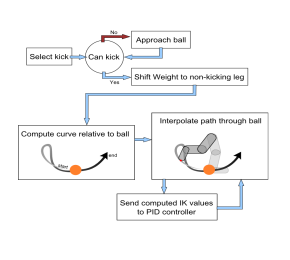
\includegraphics[scale=1]{./data/kick_arch_austin_villa}
	\caption{Schéma vykonania kopu UT Austin Villa \cite{villa2012}}
	\label{pic_kick_arch_austin_villa}
\end{figure}

Použili kubické Hermitove krivky na dosiahnutie dynamického určenia trajektórie nohy vysokou rýchlosťou od pozície lopty. Tieto krivky sa počítajú okamžite, ak vzdialenosť robota od lopty je dostatočná nato, aby sa mohol kop vykonať bez ohľadu na to, či je správne natočený. Dokážu dosiahnuť kopy do viacerých smerov. 


